% move all configuration stuff into includes file so we can focus on the content
\documentclass[aspectratio=169,hyperref={pdfpagelabels=false,colorlinks=true,linkcolor=white,urlcolor=blue},t]{beamer}

%%%%%%%%%%%%%%%%%%%%%%%%%%%%%%%%%%%%%%%%%%%%%%%%%%%%%%%%%%%%%%%%%%%%%%%%%%%%%%%%%%
%%%%%%%%%%%%%%%%%%%%%%%%%%%%%%%%%%%%%%%%%%%%%%%%%%%%%%%%%%%%%%%%%%%%%%%%%%%%%%%%%%
% packages
\usepackage{pict2e}
\usepackage{epic}
\usepackage{amsmath,amsfonts,amssymb}
\usepackage{units}
\usepackage{fancybox}
\usepackage[absolute,overlay]{textpos} 
\usepackage{media9} % avi2flv: "C:\Program Files\ffmpeg\bin\ffmpeg.exe" -i TuneFreqFilterbank.avi -b 600k -s 441x324 -r 15 -acodec copy TuneFreqFilterbank.flv
\usepackage{animate}
\usepackage{gensymb}
\usepackage{multirow}
\usepackage{silence}
\usepackage[backend=bibtex,style=ieee]{biblatex}
\AtEveryCitekey{\iffootnote{\tiny}{}}
\addbibresource{references}

%%%%%%%%%%%%%%%%%%%%%%%%%%%%%%%%%%%%%%%%%%%%%%%%%%%%%%%%%%%%%%%%%%%%%%%%%%%%%%%%%%
%%%%%%%%%%%%%%%%%%%%%%%%%%%%%%%%%%%%%%%%%%%%%%%%%%%%%%%%%%%%%%%%%%%%%%%%%%%%%%%%%%
% relative paths
\graphicspath{{graph/}}


%%%%%%%%%%%%%%%%%%%%%%%%%%%%%%%%%%%%%%%%%%%%%%%%%%%%%%%%%%%%%%%%%%%%%%%%%%%%%%%%%%
%%%%%%%%%%%%%%%%%%%%%%%%%%%%%%%%%%%%%%%%%%%%%%%%%%%%%%%%%%%%%%%%%%%%%%%%%%%%%%%%%%
% units
\setlength{\unitlength}{1mm}

%%%%%%%%%%%%%%%%%%%%%%%%%%%%%%%%%%%%%%%%%%%%%%%%%%%%%%%%%%%%%%%%%%%%%%%%%%%%%%%%%%
%%%%%%%%%%%%%%%%%%%%%%%%%%%%%%%%%%%%%%%%%%%%%%%%%%%%%%%%%%%%%%%%%%%%%%%%%%%%%%%%%%
% theme & layout
\usetheme{Frankfurt}
\beamertemplatenavigationsymbolsempty
%\setbeamertemplate{frametitle}[smoothbars theme]
\setbeamertemplate{frametitle}
{
    \begin{beamercolorbox}[ht=1.8em,wd=\paperwidth]{frametitle}
        \vspace{-.1em}%
        \hspace{.2em}{\strut\insertframetitle\strut}
        
        \hspace{.2em}\small\strut\insertframesubtitle\strut
        %\hfill
        %
\includegraphics[height=.8cm,keepaspectratio]{CenterMusicTechnology-solid-2lines-white-CoAtag}
        
    \end{beamercolorbox}
    \begin{textblock*}{100mm}(11.6cm,.7cm)
        \includegraphics[height=.8cm,keepaspectratio]{logo_GTCMT_black}
    \end{textblock*}
}

% set this to ensure bulletpoints without subsections
\usepackage{remreset}
\makeatletter
\@removefromreset{subsection}{section}
\makeatother
\setcounter{subsection}{1}

%---------------------------------------------------------------------------------
% appearance
\setbeamercolor{structure}{fg=gtgold}
\setbeamercovered{transparent} %invisible
\setbeamercolor{bibliography entry author}{fg=black}
\setbeamercolor*{bibliography entry title}{fg=black}
\setbeamercolor*{bibliography entry note}{fg=black}

%\usepackage{pgfpages}
%\setbeameroption{show notes}
%\setbeameroption{show notes on second screen=right}
%---------------------------------------------------------------------------------
% fontsize
\let\Tiny=\tiny

%%%%%%%%%%%%%%%%%%%%%%%%%%%%%%%%%%%%%%%%%%%%%%%%%%%%%%%%%%%%%%%%%%%%%%%%%%%%%%%%%%
%%%%%%%%%%%%%%%%%%%%%%%%%%%%%%%%%%%%%%%%%%%%%%%%%%%%%%%%%%%%%%%%%%%%%%%%%%%%%%%%%%
% warnings
\pdfsuppresswarningpagegroup=1
\WarningFilter{biblatex}{Patching footnotes failed}
\WarningFilter{latexfont}{Font shape}
\WarningFilter{latexfont}{Some font shapes}
\WarningFilter{gensymb}{Not defining}


%%%%%%%%%%%%%%%%%%%%%%%%%%%%%%%%%%%%%%%%%%%%%%%%%%%%%%%%%%%%%%%%%%%%%%%%%%%%%%%%%%
%%%%%%%%%%%%%%%%%%%%%%%%%%%%%%%%%%%%%%%%%%%%%%%%%%%%%%%%%%%%%%%%%%%%%%%%%%%%%%%%%%
% title information
\title[]{Introduction to Audio Content Analysis}   
\author[alexander lerch]{alexander lerch} 
%\institute{~}
%\date[Alexander Lerch]{}
\titlegraphic{\vspace{-16mm}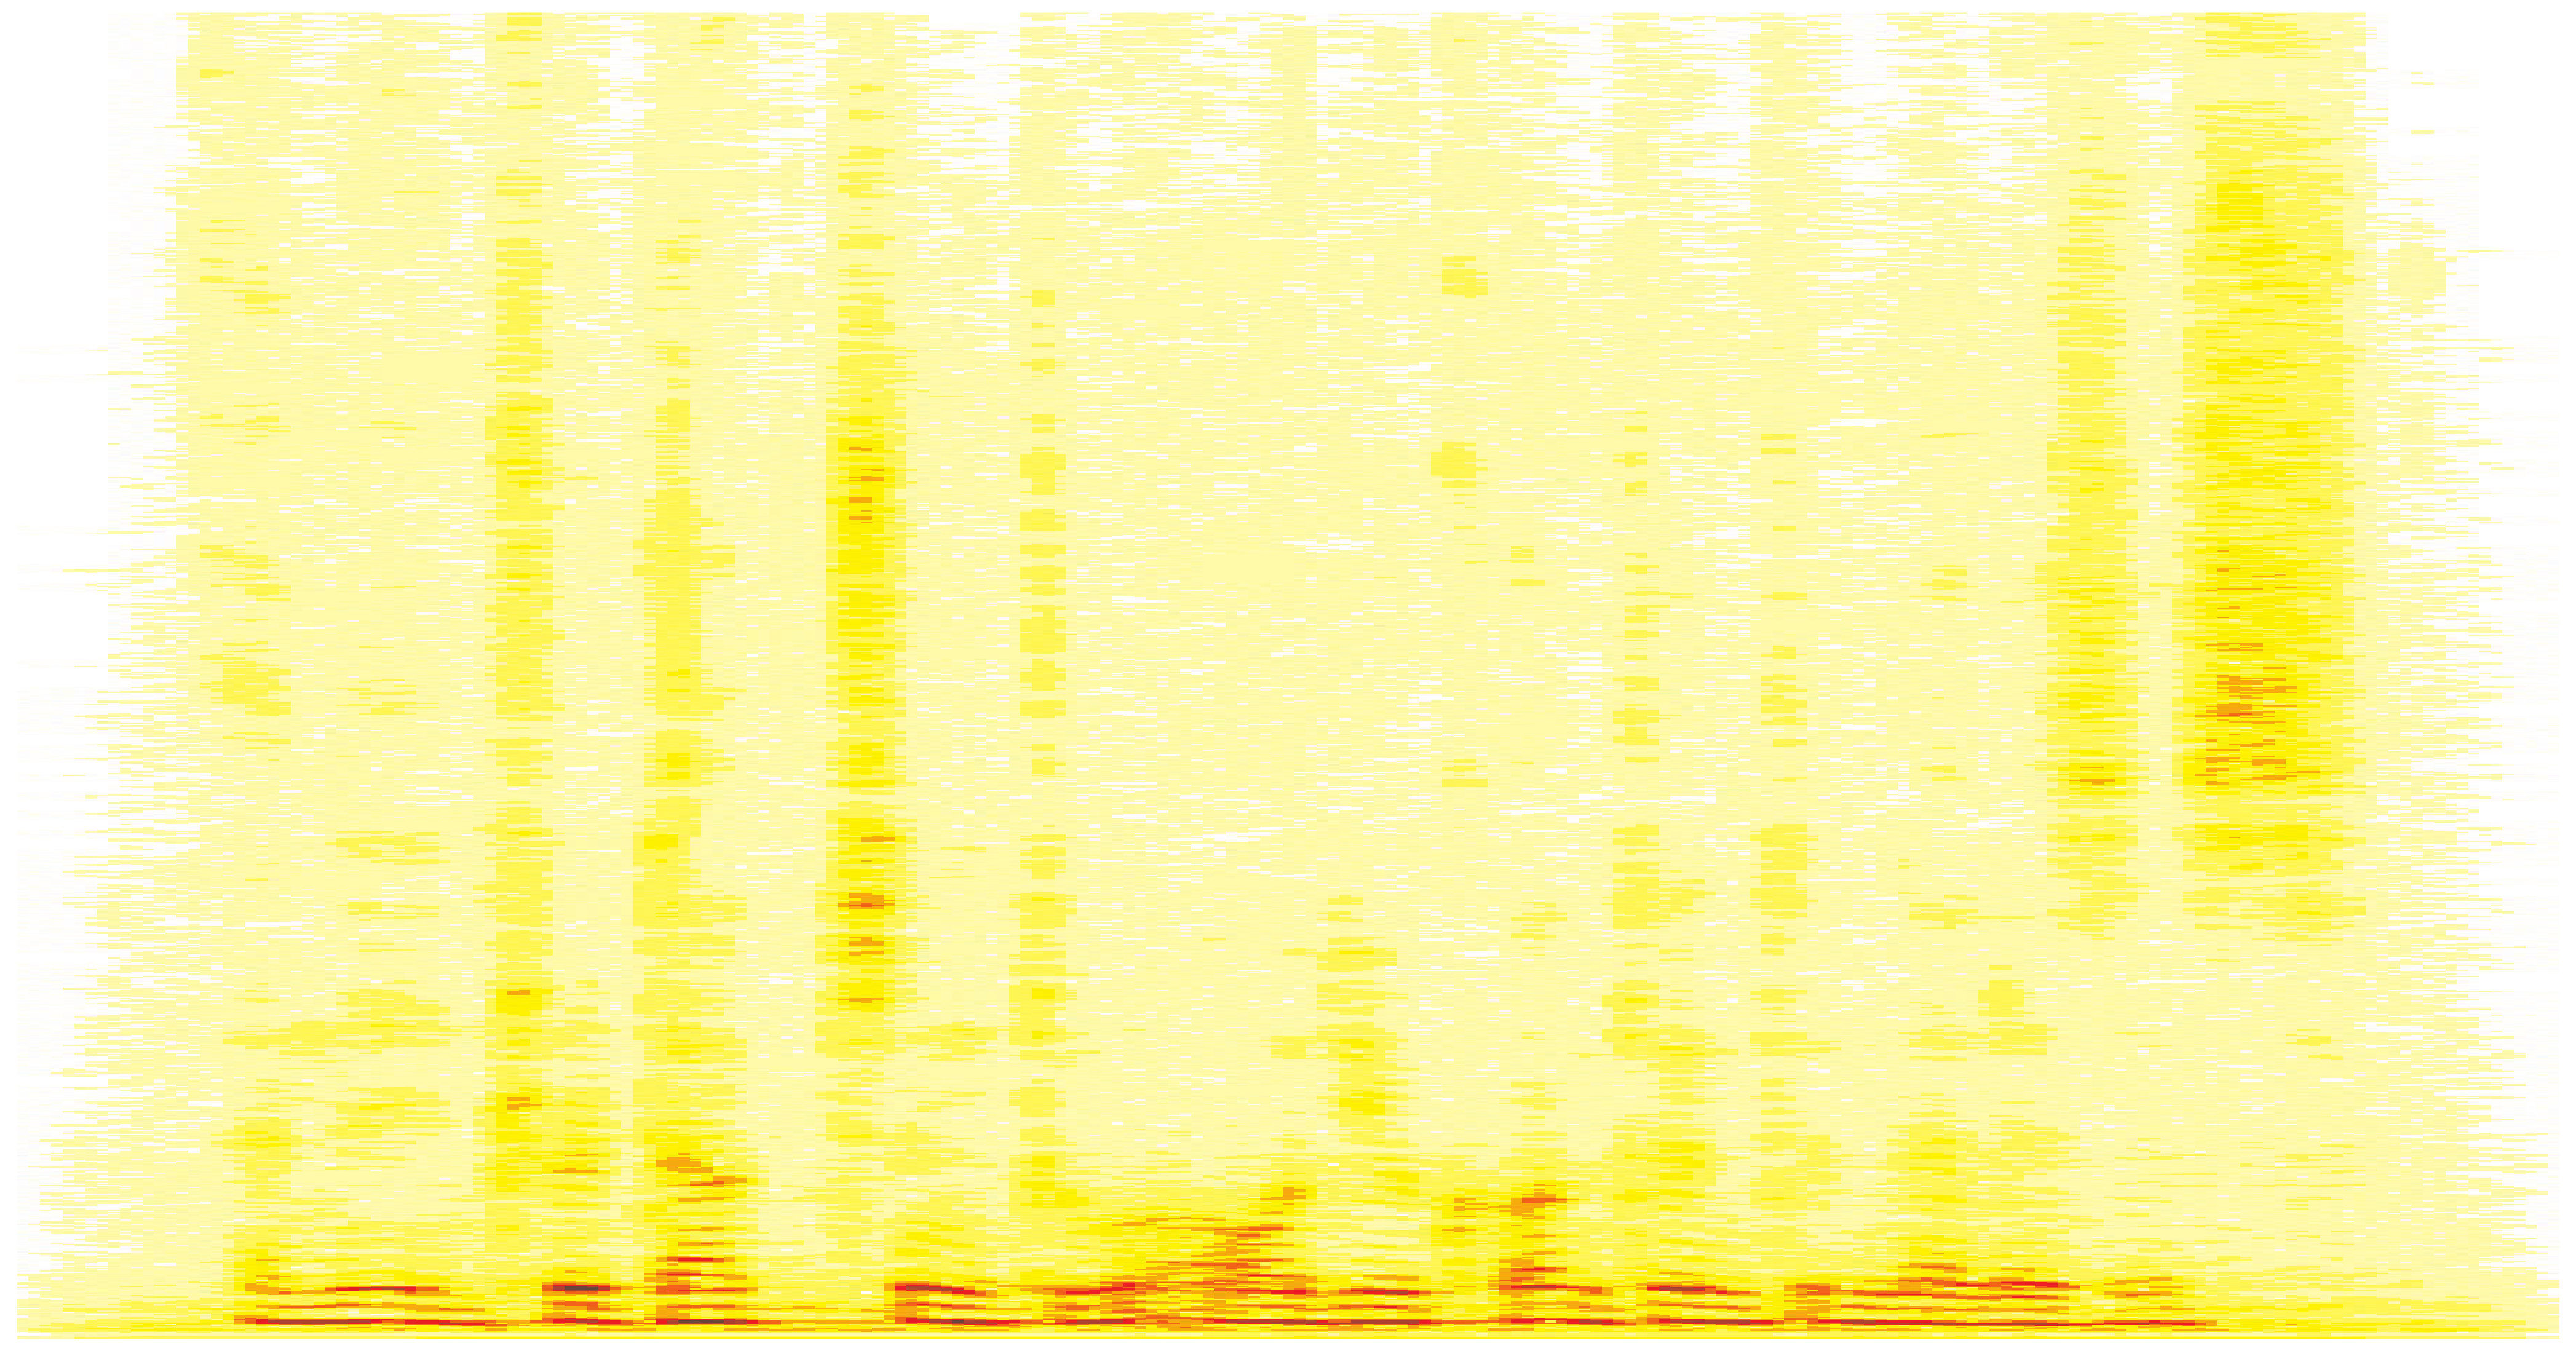
\includegraphics[width=\textwidth,height=3cm]{title}}

%%%%%%%%%%%%%%%%%%%%%%%%%%%%%%%%%%%%%%%%%%%%%%%%%%%%%%%%%%%%%%%%%%%%%%%%%%%%%%%%%%
%%%%%%%%%%%%%%%%%%%%%%%%%%%%%%%%%%%%%%%%%%%%%%%%%%%%%%%%%%%%%%%%%%%%%%%%%%%%%%%%%%
% colors
\definecolor{gtgold}{HTML}{E0AA0F} %{rgb}{0.88,0.66,1,0.06} [234, 170, 0]/256

%%%%%%%%%%%%%%%%%%%%%%%%%%%%%%%%%%%%%%%%%%%%%%%%%%%%%%%%%%%%%%%%%%%%%%%%%%%%%%%%%%
%%%%%%%%%%%%%%%%%%%%%%%%%%%%%%%%%%%%%%%%%%%%%%%%%%%%%%%%%%%%%%%%%%%%%%%%%%%%%%%%%%
% math
\DeclareMathOperator*{\argmax}{argmax}
\DeclareMathOperator*{\argmin}{argmin}
\DeclareMathOperator*{\atan}{atan}
\DeclareMathOperator*{\arcsinh}{arcsinh}
\DeclareMathOperator*{\sign}{sign}
\DeclareMathOperator*{\tcdf}{tcdf}
\DeclareMathOperator*{\si}{sinc}
\DeclareMathOperator*{\princarg}{princarg}
\DeclareMathOperator*{\arccosh}{arccosh}
\DeclareMathOperator*{\hwr}{HWR}
\DeclareMathOperator*{\flip}{flip}
\DeclareMathOperator*{\sinc}{sinc}
\DeclareMathOperator*{\floor}{floor}
\newcommand{\e}{{e}}
\newcommand{\jom}{\mathrm{j}\omega}
\newcommand{\jOm}{\mathrm{j}\Omega}
\newcommand   {\mat}[1]    		{\boldsymbol{\uppercase{#1}}}		%bold
\renewcommand {\vec}[1]    		{\boldsymbol{\lowercase{#1}}}		%bold

%%%%%%%%%%%%%%%%%%%%%%%%%%%%%%%%%%%%%%%%%%%%%%%%%%%%%%%%%%%%%%%%%%%%%%%%%%%%%%%%%%
%%%%%%%%%%%%%%%%%%%%%%%%%%%%%%%%%%%%%%%%%%%%%%%%%%%%%%%%%%%%%%%%%%%%%%%%%%%%%%%%%%
% media9
\newcommand{\includeaudio}[1]{{\includemedia[
                        addresource=audio/#1.mp3,
                        width=5mm,
                        height=5mm,
                        activate=onclick,
                        flashvars={
                            source=audio/#1.mp3  
                            &autoPlay=true
                        }]
                        {
\includegraphics[width=5mm, height=5mm]{SpeakerIcon}}
                        {APlayer.swf}}}
\newcommand{\audioautoplay}[1]{{\begin{center}\includemedia[
                            addresource=audio/#1.mp3,
                            width=.1\linewidth,
                            height=.01\linewidth,
                            activate=pageopen,
                            flashvars={
                                source=audio/#1.mp3  
                                &autoPlay=true
                            }]
                            {}
                            {APlayer.swf}\end{center}}}

\newcommand{\includevideo}[1]{{\begin{center}\includemedia[
                        addresource=video/#1.mp4,
                        width=0.8\linewidth,
                        height=0.4\linewidth,
                        activate=onclick,
                        flashvars={
                            source=video/#1.mp4  
                            &autoPlay=true
                        }]
                        {}
                        {VPlayer.swf}\end{center}}}
\newcommand{\videowithmatlab}[1]{{\begin{center}\includemedia[
                        addresource=video/animate#1.mp4,
                        width=0.8\linewidth,
                        height=0.4\linewidth,
                        activate=onclick,
                        flashvars={
                            source=video/animate#1.mp4  
                            &autoPlay=true
                        }]
                        {}
                        {VPlayer.swf}\end{center}\addreference{matlab source: matlab/animate#1.m}}}
                        

%%%%%%%%%%%%%%%%%%%%%%%%%%%%%%%%%%%%%%%%%%%%%%%%%%%%%%%%%%%%%%%%%%%%%%%%%%%%%%%%%%
%%%%%%%%%%%%%%%%%%%%%%%%%%%%%%%%%%%%%%%%%%%%%%%%%%%%%%%%%%%%%%%%%%%%%%%%%%%%%%%%%%
% other commands
\newcommand{\question}[1]{%\vspace{-4mm}
                          \setbeamercovered{invisible}
                          \begin{columns}[T]
                            \column{.8\textwidth}
                                \textbf{#1}
                            \column{.2\textwidth}
                                \vspace{-8mm}
                                \begin{flushright}
                                     
\includegraphics[scale=.5]{question_mark}
                                \end{flushright}
                                \vspace{6mm}
                          \end{columns}\pause\vspace{-12mm}}

\newcommand{\toremember}[1]{%\vspace{-4mm}
                          \begin{columns}[T]
                            \column{.8\textwidth}
                                \textbf{#1}
                            \column{.2\textwidth}
                                \vspace{-4mm}
                                \begin{flushright}
                                     
\includegraphics[scale=.5]{exclamation_mark}
                                \end{flushright}
                                \vspace{6mm}
                          \end{columns}\vspace{-6mm}}

\newcommand{\matlabexercise}[1]{%\vspace{-4mm}
                          \setbeamercovered{invisible}
                          \begin{columns}[T]
                            \column{.8\textwidth}
                                \textbf{matlab exercise}: #1
                            \column{.2\textwidth}
                                \begin{flushright}
                                     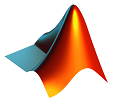
\includegraphics[scale=.5]{logo_matlab}
                                \end{flushright}
                                %\vspace{6mm}
                          \end{columns}}

\newcommand{\addreference}[1]{  
                  
                    \begin{textblock*}{\baselineskip }(1.12\textwidth,.3\textheight) %(1.15\textwidth,.4\textheight)
                        \rotatebox{90}{\tiny {#1}}
                    \end{textblock*}}
                    
\newcommand{\figwithmatlab}[1]{
                    \begin{figure}
                        \centering
                        \includegraphics{#1}
                        %\label{fig:#1}
                    \end{figure}
                    
                    \addreference{matlab source: \href{https://github.com/alexanderlerch/ACA-Slides/blob/master/matlab/display#1.m}{matlab/display#1.m}}}
\newcommand{\figwithref}[2]{
                    \begin{figure}
                        \centering
                        \includegraphics{#1}
                        \label{fig:#1}
                    \end{figure}
                    
                    \addreference{#2}}  
                                    
\newcommand{\inserticon}[1]{

                    \begin{textblock*}{100mm}(14.5cm,7.5cm)
                        \includegraphics[height=.8cm,keepaspectratio]{#1}
                    \end{textblock*}}            

%%%%%%%%%%%%%%%%%%%%%%%%%%%%%%%%%%%%%%%%%%%%%%%%%%%%%%%%%%%%%%%%%%%%%%%%%%%%%%%%%%
%%%%%%%%%%%%%%%%%%%%%%%%%%%%%%%%%%%%%%%%%%%%%%%%%%%%%%%%%%%%%%%%%%%%%%%%%%%%%%%%%%
% counters
\newcounter{i}
\newcounter{j}
\newcounter{iXOffset}
\newcounter{iYOffset}
\newcounter{iXBlockSize}
\newcounter{iYBlockSize}
\newcounter{iYBlockSizeDiv2}
\newcounter{iDistance}


\newcommand{\listspectralfeature}[2]{
\vspace{-6mm}
\begin{footnotesize}
\begin{equation*}
    \input{eq/Spectral#1}
\end{equation*}
\end{footnotesize}
\only<1>{
    {\flushright\includeaudio{sax_example}}
    \vspace{-9mm}
    \figwithref{FeaturesSpectral#1}{matlab source: \href{https://github.com/alexanderlerch/ACA-Slides/blob/master/matlab/displayFeatures.m}{matlab/displayFeatures.m}}
    \inserticon{audio}
}
\only<2>{
    %\vspace{10mm}
    
    \textbf{common variants}:
    
    {#2}
    }
}                    


\subtitle{Module 3.3: Feature Extraction~---~Additional (Instantaneous) Features}

%%%%%%%%%%%%%%%%%%%%%%%%%%%%%%%%%%%%%%%%%%%%%%%%%%%%%%%%%%%%%%%%%%%%%%%%%%%%
\begin{document}
    % generate title page
	

\begin{frame}
    \titlepage
    %\vspace{-5mm}
    \begin{flushright}
        \href{http://www.gtcmt.gatech.edu}{\includegraphics[height=.8cm,keepaspectratio]{logo_GTCMT_black}}
    \end{flushright}
\end{frame}


    \section[overview]{lecture overview}
        \begin{frame}{introduction}{overview}
            \begin{block}{corresponding textbook section}
                    \href{http://ieeexplore.ieee.org/xpl/articleDetails.jsp?arnumber=6331120}{Chapter 3~---~Instantaneous Features}: pp.~54--63
            \end{block}

            \begin{itemize}
                \item   \textbf{lecture content}
                    \begin{itemize}
                        \item   tonalness features: describing ratio of tonal vs.\ noisy   
                        \item   technical features: describing basic signal properties
                        \item   quick introduction to feature learning
                    \end{itemize}
                \bigskip
                \item<2->   \textbf{learning objectives}
                    \begin{itemize}
                        \item   summarize features, describe their computation, and discuss their meaning
                        \item   discuss advantages and disadvantages of feature learning as opposed to custom-designed features
                    \end{itemize}
            \end{itemize}
            \inserticon{directions}
        \end{frame}

    \section[tonalness]{tonalness features}
        \begin{frame}{tonalness features}{spectral crest factor}
            \listspectralfeature{CrestFactor}{\begin{itemize}   \item normalization \item power spectrum \item measure \textit{per band} instead of  whole spectrum \end{itemize}}
        \end{frame}
        \begin{frame}{tonalness features}{spectral flatness}
            \listspectralfeature{Flatness}{\begin{itemize}   \item power vs.\ magnitude spectrum \item smoothed spectrum (avoid spurious 0-bins) \item measure \textit{per band} instead of  whole spectrum \end{itemize}}
        \end{frame}
        \begin{frame}{tonalness features}{spectral tonal power ratio}
            \listspectralfeature{TonalPowerRatio}{\begin{itemize}   \item definition of tonal/non-tonal components \end{itemize}}
        \end{frame}
        
		\begin{frame}{tonalness features}{maximum of ACF}
            \vspace{-6mm}
			\begin{equation*}
				v_{\mathrm{Ta}}(n)	= \max\limits_{0\leq \eta \leq \mathcal{K}-1}{|r_{xx}(\eta,n)|}
			\end{equation*}
            {\flushright\includeaudio{sax_example}}
            \vspace{-9mm}
            \inserticon{audio}
            \figwithref{FeaturesTimeMaxAcf}{matlab source: \href{https://github.com/alexanderlerch/ACA-Slides/blob/master/matlab/displayFeatures.m}{matlab/displayFeatures.m}}
		\end{frame}
		%\begin{frame}{tonalness features}{maximum of ACF 2/2}
            %\question{maximum detection: how to avoid main lobe maxima?}
			%
			%\begin{itemize}
				%\item	minimum lag
				%\item	magnitude threshold
				%\item	search only after first local minimum
			%\end{itemize}
		%\end{frame}
        %Predictivity Ratio
        %SpectralPredictivity

    \section[technical]{technical properties}
		\begin{frame}{technical features}{zero crossing rate}
            \vspace{-6mm}
			\begin{equation*}\label{eq:zc}
				v_{\mathrm{ZC}}(n) = \frac{1}{2 \cdot\mathcal{K}}\sum\limits_{i=i_{\mathrm{s}}(n)}^{i_{\mathrm{e}}(n)}{\big|\sign \left[x(i)\right]-\sign \left[x(i-1)\right]\big|} 
			\end{equation*}
            {\flushright\includeaudio{sax_example}}
            \vspace{-9mm}
            \inserticon{audio}
            \figwithref{FeaturesTimeZeroCrossingRate}{matlab source: \href{https://github.com/alexanderlerch/ACA-Slides/blob/master/matlab/displayFeatures.m}{matlab/displayFeatures.m}}
		\end{frame}
		\begin{frame}{technical features}{ACF coefficients}
            \vspace{-6mm}
			\begin{equation*}
				v^{\eta}_{\mathrm{ACF}}(n)	= r_{xx}(\eta,n) \quad \text{with}\enspace \eta = 1,2,3,\ldots
			\end{equation*}
            {\flushright\includeaudio{sax_example}}
            \vspace{-9mm}
            \inserticon{audio}
            \figwithref{FeaturesTimeAcfCoeff}{matlab source: \href{https://github.com/alexanderlerch/ACA-Slides/blob/master/matlab/displayFeatures.m}{matlab/displayFeatures.m}}
		\end{frame}

    \section[learned]{feature learning}
        \begin{frame}{feature learning}{introduction}
            \begin{itemize}
                \item   \textbf{hand-crafted features}:
                    \begin{itemize}
                        \item   arbitrary definitions
                        \item   simple to compute
                        \item   mostly focus on one technical property
                        \item   provide limited information
                    \end{itemize}
                    
                \bigskip
                \item<2-> \textbf{feature learning}:
                    \begin{itemize}
                        \item   \textit{automatically} learn features from data-set
                        \item   meaning not obvious, can combine multiple properties
                        
                    \end{itemize}
            \end{itemize}
		\end{frame}
        \begin{frame}{feature learning}{overview}
            \begin{itemize}
                \item   \textbf{principle}
                    \begin{enumerate}
                        \item   put (a lot of) raw data at input
                        \item   learn a way of reducing dimensionality while keeping as much information as possible
                    \end{enumerate}
                \bigskip
                \item<2->   \textbf{advantages}
                    \begin{itemize}
                        \item   features might contain more useful information than provided by hand-crafted features
                        \item   no expert knowledge required
                        %\item   possibly easier generalization
                    \end{itemize}
                \smallskip
                \item<3->   \textbf{disadvantages}
                    \begin{itemize}
                        \item   usually time consuming
                        \item   limited ways of controlling the type of information learned
                    \end{itemize}
            \end{itemize}
		\end{frame}
        \begin{frame}{feature learning}{approaches 1/2}
            \begin{itemize}
                \item   \textbf{dictionary learning} (sparse coding, non-negative matrix factorization)
                    \begin{equation*}
                        X = B\cdot A
                    \end{equation*}
                    \begin{itemize}
                        \item[]   $X$: input signal to be modeled (often spectrogram)
                        \item[]   $B$: dictionary/template matrix (often set of single spectra that comprise the basic building blocks of $X$)
                        \item[]   $A$: activation matrix indicating the weight and superposition of templates 
                    \end{itemize}
                    \begin{itemize}
                        \item   derive $B$,$A$, by minimizing a cost function, e.g. $||X-BA||_2$
                    \end{itemize}
                \item<2->[$\rightarrow$] templates are trained, activations are used as feature vector (length: number of templates)
            \end{itemize}
		\end{frame}
        \begin{frame}{feature learning}{approaches 2/2}
            \begin{itemize}
                \item   \textbf{clustering} 
                    \begin{itemize}
                        \item   find clusters in data set (e.g., from magnitude spectra or simple features)
                        \item   store median of clusters (compare: template matrix)
                        \smallskip
                        \item<2->[$\rightarrow$]   features:
                            \begin{itemize}
                                \item   binary vector (length: number of clusters, zero except for closest cluster)
                                \item   distance vector (distance to each cluster)
                            \end{itemize}
                    \end{itemize}
                \bigskip
                \item<3->   neural networks and \textbf{deep architectures} 
                    \begin{itemize}
                        \item   stack multiple layers of simple learning blocks
                        \item   each layer uses the output of the previous layer as input
                        \smallskip
                        \item<4->[$\rightarrow$]   feature: output of the highest layer
                    \end{itemize}
            \end{itemize}
		\end{frame}
        \begin{frame}{instantaneous features}{matlab exercise}
            \matlabexercise{spectral centroid}
            \begin{footnotesize}
            \begin{enumerate}
                \item   implement a function extracting the spectral centroid from a magnitude spectrum
                    \begin{itemize}
                        \item   use the following interface (output is one value)\\ \begin{scriptsize}\texttt{[v\_SC] = SpectralCentroid(MagSpec)}\end{scriptsize}
                        \item   consider:
                            \begin{enumerate}
                                \item   what tests do you implement to verify your implementation
                                \item   what additional code to avoid undefined outputs
                            \end{enumerate}
                    \end{itemize}
                \item   implement a caller function reading an audio file and extracting the Spectral Centroid for each block using the function above
                    \begin{itemize}
                        \item   use the following interface (output is vector)\\ \begin{scriptsize}\texttt{[v\_SC,tInS] = extractSpectralCentroid(Path2AudioFile, BlockSize, HopSize)}\end{scriptsize}
                        %\item   consider:
                            %\begin{itemize}
                                %\item   what to do with start and end blocks
                                %\item   how to handle user inconsistencies (invalid path, hopsize larger than blocksize, ...)
                            %\end{itemize}
                    \end{itemize}
            \end{enumerate}
            \end{footnotesize}
       \end{frame}

        
    \section{summary}
        \begin{frame}{summary}{lecture content}
            \begin{itemize}
                \item   \textbf{tonalness features}
                    \begin{itemize}
                        \item   in many cases closely related to spectral shape features
                        \item   low level instantaneous features trying to estimate the ratio of tonal vs.\ noisy
                    \end{itemize}
                \bigskip
                \item   \textbf{technical features}
                    \begin{itemize}
                        \item   implementing a technical signal description that might or might not be interpretable
                        \item   in many cases only of limited use
                    \end{itemize}
                \bigskip
                \item   \textbf{feature learning}
                    \begin{itemize}
                        \item   data-driven approach without expert knowledge
                        \item   can be very powerful in the right context with enough representative data
                    \end{itemize}
            \end{itemize}
            \inserticon{summary}
        \end{frame}
\end{document}
